\chapter{Descripción del Trabajo}
\label{cap:descripcionTrabajo}

%  Aquí comienza la descripción del trabajo realizado. Se deben incluir tantos capítulos como sea necesario para describir de la manera más completa posible el trabajo que se ha llevado a cabo. Como muestra la figura \ref{fig:sampleImage}, está todo por hacer.

% \begin{figure}[h]
% 	\centering
% 	
\includegraphics[width = 0.5\textwidth]{Imagenes/Vectorial/Todo.pdf}
% 	\caption{Ejemplo de imagen}
% 	\label{fig:sampleImage}
% \end{figure}

% Si te sirve de utilidad,  puedes incluir tablas para mostrar resultados, tal como se ve en la tabla \ref{tab:sampleTable}.


% \begin{table}
% 	\centering
% 	\begin{tabular}{c|c|c}
% 		\textbf{Col 1} & \textbf{Col 2} & \textbf{Col 3} \\
% 		\hline\hline
% 		3 & 3.01 & 3.50\\
% 		6 & 2.12 & 4.40\\
% 		1 & 3.79 & 5.00\\
% 		2 & 4.88 & 5.30\\
% 		4 & 3.50 & 2.90\\
% 		5 & 7.40 & 4.70\\
% 		\hline
% 	\end{tabular}
% 	\caption{Tabla de ejemplo}
% 	\label{tab:sampleTable}
% \end{table}
\chapterquote{El número 42.}{Guía del autoestopista galáctico - Douglas Adams}
El trabajo descrito en este capítulo es un plugin para \textit{OBS Studio} que convierte cualquier retransmisión de vídeo en una experiencia de realidad aumentada orientada a concursos de programación. El plugin detecta marcadores \textbf{ArUco} \citep{GarridoJurado2014} impresos sobre las mesas del concurso, estima su posición y orientación exactas en el espacio real, y sobre ese anclaje físico superpone contenido virtual: modelos 3D arbitrarios, un cronómetro analógico sincronizado con el servidor del juez, y paneles de texto con la clasificación general o los datos del equipo que la cámara está captando en ese momento. Todo ello ocurre en tiempo real dentro del propio pipeline de vídeo de \textit{OBS Studio}, sin software externo ni procesado adicional, de modo que el operador gestiona el sistema desde el mismo panel con el que controla el resto de la retransmisión.

Siguiendo la taxonomía descrita en el capítulo anterior, el sistema encaja en tres categorías de la clasificación de la RA. Es \textbf{marker-based}: el anclaje del contenido virtual al mundo físico se basa en los marcadores ArUco impresos en las mesas, sin necesidad de reconstrucción del entorno ni de sensores adicionales. Es \textbf{video see-through}: la imagen del mundo real se captura mediante la cámara del equipo de retransmisión y el contenido virtual se dibuja sobre ella antes de emitirse. Y es \textbf{RA aditiva}: los elementos virtuales se superponen a la escena sin reemplazar ningún elemento real, enriqueciendo la imagen sin alterar lo que hay debajo. Esta combinación es la más habitual en contextos de retransmisión profesional, donde el operador necesita ver siempre el vídeo real junto con los gráficos añadidos.

El desarrollo cubre tres grandes áreas técnicas. La primera es el motor de renderizado 3D integrado en OBS, capaz de cargar modelos en múltiples formatos, aplicar cadenas de transformaciones espaciales y animar las manecillas del cronómetro fotograma a fotograma. La segunda es el sistema de visión por computador, basado en \textbf{OpenCV} y en una calibración previa de la cámara, que resuelve en tiempo real la posición y orientación de cada marcador respecto a la lente. La tercera es la capa de conectividad asíncrona que, mediante \textbf{libcurl}, mantiene sincronizados los datos del concurso con la API de \textbf{DOMjudge} sin interferir en ningún momento con el hilo de renderizado.


\section{Construcción y ciclo de vida}

El desarrollo del plugin requiere una infraestructura que gestione dependencias multiplataforma y garantice un rendimiento estable en tiempo real dentro de OBS Studio.

\subsection{Dependencias y compilación}

Se utiliza \textbf{CMake} como sistema de construcción debido a su capacidad para generar archivos de proyecto nativos en Windows, macOS y Linux. La configuración se apoya en los siguientes elementos clave:

\begin{itemize}
    \item \textbf{CMakePresets:} Define perfiles de compilación estándar (\textit{Debug, Release}), unificando los parámetros de compilación para todos los desarrolladores.
    \item \textbf{Buildspec:} Archivo de metadatos que especifica la versión del plugin, la versión mínima de la API de OBS y la identificación del módulo.
    \item \textbf{Gestión de dependencias:} El proyecto integra tres bibliotecas fundamentales:
    \begin{itemize}
        \item \textbf{OpenCV:} Para el procesamiento de imágenes y la lógica de detección ArUco.
        \item \textbf{ASSIMP:} Para la importación y normalización de modelos 3D en múltiples formatos (OBJ, FBX, COLLADA, entre otros).
        \item \textbf{libcurl:} Para la comunicación mediante peticiones HTTP REST.
    \end{itemize}
\end{itemize}

\subsection{Ciclo de vida del plugin}

El ciclo de ejecución se rige por el modelo de eventos de OBS Studio, dividiéndose en tres fases principales:

\subsubsection{Inicialización}
En esta fase se reserva la memoria para la estructura  y se preparan los recursos gráficos:
\begin{enumerate}
    \item \textbf{Carga de Shaders:} Compilación de los programas de GPU necesarios para el renderizado.
    \item \textbf{Inicialización AR:} Carga de los parámetros de calibración de la cámara y configuración del diccionario ArUco.
    \item \textbf{Recursos 3D:} Carga inicial de mallas y texturas en la memoria de vídeo (VRAM).
\end{enumerate}



\begin{figure}[H] %% La H mayúscula fuerza la posición exacta
    \centering
    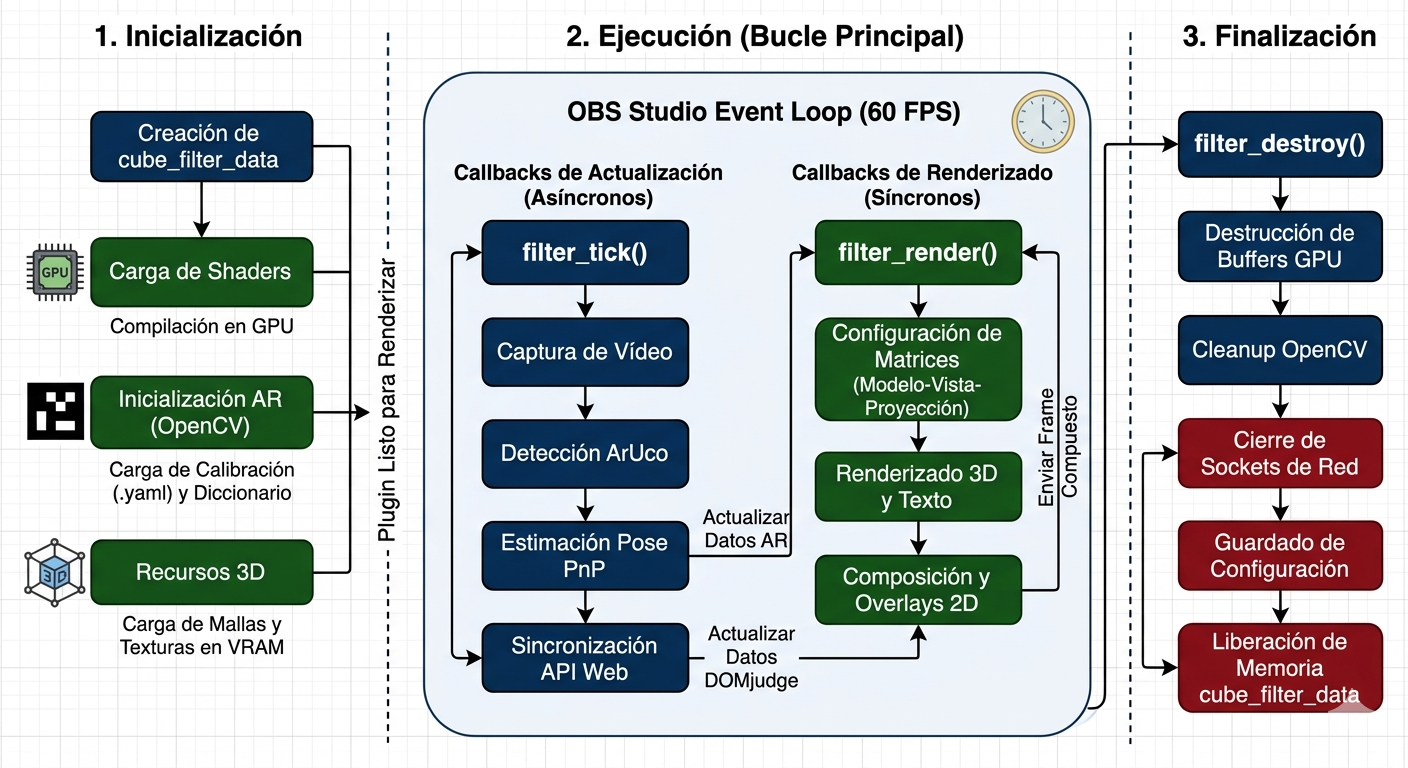
\includegraphics[width=0.8\linewidth]{Imagenes/Vectorial/ciclo_vida_plugin}
    \caption{Diagrama detallado del ciclo de vida del plugin}
    \label{fig:ciclo_vida_plugin}
\end{figure}



\subsubsection{Actualización de lógica}
Este \textit{callback} se ejecuta en cada cuadro (\textit{frame}) para actualizar el estado interno sin bloquear el renderizado:
\begin{itemize}
    \item \textbf{Detección:} Captura del frame de vídeo, conversión a espacio de color BGR y búsqueda de marcadores ArUco.
    \item \textbf{Sincronización:} Procesamiento asíncrono de los datos recibidos vía Web.
    \item \textbf{Cálculo de Pose:} Estimación de la posición y rotación de los objetos 3D basada en los marcadores detectados.
\end{itemize}

\subsubsection{Renderizado gráfico}
Es la etapa donde se genera la salida visual final. El flujo de trabajo sigue este orden:
\begin{enumerate}
    \item Configuración del \textit{Z-buffer} para la gestión de profundidad.
    \item Aplicación de matrices de transformación (Modelo-Vista-Proyección).
    \item Dibujo de la geometría 3D sobre el flujo de vídeo original de OBS.
    \item Superposición (\textit{Overlay}) de elementos 2D como el marcador de puntuación o el reloj.
\end{enumerate}

\subsection{Configuración dinámica}

El plugin permite la modificación de parámetros en tiempo de ejecución sin necesidad de reiniciar la fuente de vídeo. Cuando el usuario modifica una propiedad en la interfaz de OBS, el sistema activa una recarga selectiva:
\begin{itemize}
    \item \textbf{Recarga de modelos:} Si cambia la ruta del archivo, se libera la memoria anterior y se carga la nueva geometría mediante ASSIMP.
    \item \textbf{Ajuste de Offsets:} Los cambios en la posición o escala manual se aplican inmediatamente a las matrices de transformación del siguiente frame.
    \item \textbf{Calibración:} Permite ajustar los umbrales de detección AR para adaptarse a diferentes condiciones de iluminación en directo.
\end{itemize}

\subsection{Arquitectura de hilos}
\label{subsec:hilos}

El plugin separa las responsabilidades en dos contextos de ejecución para garantizar que ninguna operación costosa bloquee la salida de vídeo.

El \textbf{hilo principal} es gestionado íntegramente por OBS Studio. Sobre él recaen los tres tipos de \textit{callbacks} que el plugin registra. El callback de vídeo recibe cada fotograma entrante y ejecuta la detección ArUco. El callback de renderizado construye la salida visual final fotograma a fotograma. Las actualizaciones de la interfaz de usuario se producen cuando el operador modifica algún parámetro en el panel de propiedades. Dado que los tres comparten el mismo hilo, la implementación evita cualquier operación bloqueante dentro de ellos, pues la detección ArUco debe completarse en menos de un fotograma y el renderizado no puede esperar datos de red.

El \textbf{hilo secundario} lo crea el propio plugin al activarse la conectividad web, mediante una llamada a \texttt{CreateThread} de la API de Windows. Este hilo ejecuta un bucle que lanza peticiones HTTP a DOMjudge a intervalos configurables, duerme entre consultas y escribe los resultados en una estructura compartida protegida por una \texttt{CRITICAL\_SECTION}. De este modo el hilo principal únicamente lee el último resultado disponible sin bloquear el renderizado, y cuando el plugin se destruye se señaliza al hilo secundario para que termine de forma limpia antes de liberar los recursos.

\begin{figure}[H]
\centering
\begin{tikzpicture}[>=stealth, font=\small, node distance=1.2cm]
  \node[draw, rounded corners, fill=blue!8, minimum width=5.5cm, minimum height=1cm, align=center]
    (main) {\textbf{Hilo principal (OBS)}\\{\scriptsize vídeo · renderizado · UI}};
  \node[draw, rounded corners, fill=orange!10, minimum width=5.5cm, minimum height=1cm, align=center,
    below=1.6cm of main]
    (sec) {\textbf{Hilo secundario (plugin)}\\{\scriptsize peticiones HTTP · libcurl}};
  \draw[<->, thick] (main) -- node[right, align=left, font=\scriptsize]
    {\texttt{CRITICAL\_SECTION}\\resultado en caché}
    (sec);
\end{tikzpicture}
\caption{Arquitectura de dos hilos del plugin. El hilo principal de OBS gestiona renderizado y detección; el hilo secundario realiza las peticiones HTTP de forma asíncrona.}
\label{fig:hilos}
\end{figure}

\section{Modelos 3D y overlays}

La visualización de elementos virtuales requiere un sistema capaz de procesar geometría compleja en tiempo real, manteniendo la coherencia espacial con el entorno capturado.

\subsection{Gestión de geometría poligonal}

El módulo \texttt{SJ\_3DModel} centraliza la lógica de importación y dibujo de objetos. La carga se delega en la biblioteca \textbf{ASSIMP}, que admite múltiples formatos de modelo 3D (\textit{OBJ, FBX, COLLADA}, entre otros), abstrayendo al plugin de los detalles de cada formato y exponiendo siempre la misma estructura de malla normalizada.

\subsubsection{Estructura de malla}
Cada modelo se descompone en una o varias mallas, definidas por:
\begin{itemize}
    \item \textbf{Vertex Buffer:} Almacena las coordenadas $(x, y, z)$, vectores normales para iluminación y coordenadas UV para el mapeo de texturas.
    \item \textbf{Index Buffer:} Define la conectividad de los vértices para formar triángulos, optimizando el uso de memoria GPU.
    \item \textbf{Materiales:} Referencias a texturas externas y propiedades de reflexión de la superficie.
\end{itemize}

\cuadro{
\begin{tabular}{lp{5cm}l}
\toprule
\textbf{Componente} & \textbf{Atributos contenidos} & \textbf{Ubicación} \\ \midrule
\textit{Vertex Buffer} & Posición (XYZ),(RGB), UV & VRAM (GPU) \\
\textit{Index Buffer} & Orden Dibujado de triángulos & VRAM (GPU) \\
\textit{Materiales} & Texturas y Shaders & Memoria RAM/GPU \\ \bottomrule
\end{tabular}}


\subsection{Transformaciones y control de usuario}

Para posicionar los modelos, el sistema utiliza \textbf{matrices de transformación homogéneas 4x4}. Estas permiten encadenar traslación, rotación y escala en una sola operación matricial:
\[ M = T \cdot R \cdot S \]

\begin{itemize}
    \item \textbf{Rotación (Pitch, Yaw, Roll):} El usuario puede ajustar la orientación manual mediante ángulos de Euler, que internamente se combinan con la matriz de pose calculada por el detector ArUco.
    \item \textbf{Cálculo de Pivotes:} El sistema calcula automáticamente el \textit{Bounding Box} del modelo para situar el centro de rotación en la base o centro geométrico del objeto, evitando rotaciones excéntricas.
    \item \textbf{Escalado Dinámico:} Se implementa un factor de escala global para ajustar el tamaño del modelo virtual al tamaño físico del marcador de referencia.
\end{itemize}



\subsection{Texto 3D y overlays}

El plugin incorpora un motor de renderizado de texto para mostrar información contextual (como el cronómetro o puntuaciones) directamente en la escena.

\subsubsection{Texto proyectado en 3D}
El cronómetro, el nombre del equipo o cualquier otro texto informativo que el plugin muestra no flota fijo en pantalla: se mueve y gira con el marcador como si estuviera impreso sobre él. Para lograrlo, el sistema calcula en cada fotograma la orientación exacta del marcador en el espacio y aplica esa misma orientación al bloque de texto antes de dibujarlo. El resultado es que si el marcador se inclina hacia la cámara el texto se inclina con él, y si gira sobre la mesa el texto gira también. El efecto da la sensación de que la información está físicamente anclada al marcador, aunque en realidad se recalcula y se redibuja en cada fotograma a partir de la pose detectada.

\subsection{El modo cronómetro 3D}
\label{subsec:countdown}

El plugin incluye un modo de visualización dedicado al cronómetro de la competición, en el que el modelo 3D renderizado sobre el marcador actúa como un reloj analógico de cuenta atrás. Su propósito es mostrar el tiempo restante del concurso de forma visualmente llamativa, anclado sobre la mesa del jurado o en cualquier punto de la escena.

La lógica del cronómetro reside en el módulo \texttt{countdown\_clock}, que mantiene el estado de la cuenta atrás (\texttt{STOPPED}, \texttt{RUNNING}, \texttt{PAUSED} o \texttt{FINISHED}), la duración total configurada en horas, minutos y segundos, y el tiempo restante que se decrementa fotograma a fotograma. En cada iteración del callback de vídeo el sistema llama a \texttt{countdown\_clock\_tick} con el tiempo transcurrido desde el frame anterior, lo que actualiza el tiempo restante con alta precisión independientemente de la cadencia de fotogramas.

El tiempo restante se traduce en ángulos de rotación para las mallas 3D de las manecillas. El plugin ofrece dos modos de presentación:

\begin{itemize}
    \item \textbf{Tres manecillas:} Cada malla del modelo (hora, minuto y segundo) recibe su propio ángulo calculado de forma análoga a un reloj analógico. La manecilla de segundos avanza $6°$ por segundo, la de minutos $6°$ por minuto completado y la de horas divide proporcionalemente el rango configurado del cuadrante.
    \item \textbf{Manecilla única:} Una sola malla barre $360°$ a lo largo de la duración total del concurso, de modo que su posición angular representa qué fracción del tiempo total ha transcurrido, como un indicador de progreso circular.
\end{itemize}

La posición del reloj puede fijarse manualmente en pantalla o anclarse a un marcador ArUco, de la misma forma que el modelo 3D estándar. Cuando la conectividad con DOMjudge está activa, el tiempo restante se sincroniza periódicamente con el valor que reporta el servidor mediante \texttt{countdown\_clock\_sync\_full}, corrigiendo cualquier deriva acumulada por el reloj local y garantizando que el cronómetro sea siempre coherente con el estado oficial del concurso.

\section{Detección ArUco y calibración de cámara}
s
La fidelidad de la Realidad Aumentada depende de la capacidad del sistema para traducir coordenadas de píxeles (2D) a una posición en el espacio real (3D). Este proceso se apoya en el uso de marcadores ArUco y una calibración precisa de la cámara.

\subsection{Integración con OpenCV}

De entre las bibliotecas y SDKs analizados en el capítulo anterior, se ha elegido \textbf{OpenCV} como motor de visión por computador. ARToolKit, el precursor histórico del tracking por marcadores, habría sido una alternativa conceptualmente cercana, pero su mantenimiento activo es limitado y carece de soporte nativo para diccionarios ArUco modernos. Vuforia ofrece tracking de marcadores robusto, pero está orientada a Unity y a plataformas móviles, e impone restricciones de licencia incompatibles con un plugin de código abierto. OpenCV, en cambio, es gratuita, multiplataforma, dispone de soporte oficial para marcadores ArUco dentro de su módulo \texttt{objdetect}, y se integra directamente con C sin depender de ningún motor externo, lo que la hace idónea para un plugin nativo de OBS.

Para gestionar la detección se ha desarrollado el módulo \texttt{aruco\_detector}, que actúa como capa de abstracción sobre la API de OpenCV y expone funciones simplificadas al plugin:

\begin{itemize}
    \item  Analiza el fotograma de OBS en busca de patrones binarios.
    \item  Calcula la traslación y rotación del marcador respecto a la lente.
    \item  Permite seleccionar el diccionario de códigos de detección ArUco desde la interfaz de preferencias de OBS.
\end{itemize}

\subsection{Calibración de la cámara}

Cada cámara de vídeo posee imperfecciones ópticas (distorsión radial y tangencial) que curvan la imagen. Para corregirlas, se aplica un modelo matemático de calibración:

\begin{itemize}
    \item \textbf{Matriz Intrínseca ($K$):} Define la distancia focal y el punto principal del sensor. Es vital para que el tamaño del objeto 3D sea coherente con la distancia real.
    \item \textbf{Coeficientes de Distorsión:} Permiten corregir las deformaciones geométricas que introducen las lentes reales, de modo que los objetos 3D se proyecten con precisión sobre la imagen sin desviaciones perceptibles en los bordes del encuadre.
\end{itemize}

El sistema carga estos parámetros desde un archivo generado previamente mediante un proceso de calibración con tablero de ajedrez. La figura~\ref{fig:modelo_pinhole} ilustra el modelo geométrico que justifica esta calibración.

\begin{figure}[H]
    \centering
    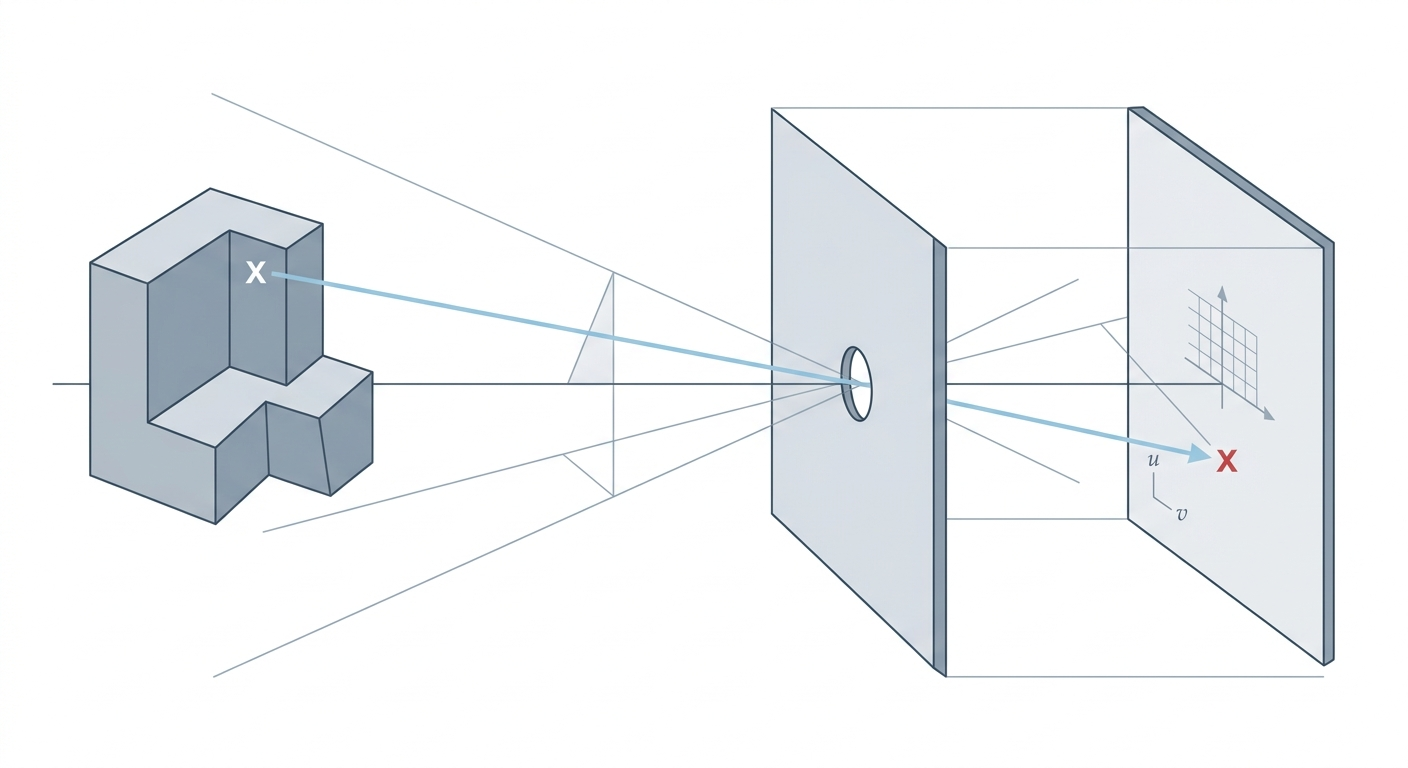
\includegraphics[width=0.6\textwidth]{Imagenes/Vectorial/CamaraDistorsion}
    \caption{Diagrama geométrico del modelo de cámara \textit{pinhole}. Un punto $P$ en el espacio real se proyecta a través del centro óptico hasta el plano del sensor, produciendo la coordenada de píxel $(u,v)$. La calibración corrige las desviaciones que introducen las lentes reales respecto a este modelo ideal.}
    \label{fig:modelo_pinhole}
\end{figure}

\subsubsection{Proceso de calibración}

El proyecto incluye una herramienta de calibración propia formada por el script Python \texttt{calibrate.py} y el lanzador \texttt{calibrate.bat} para Windows. El proceso consta de tres pasos:

\begin{enumerate}
    \item \textbf{Toma de fotografías:} El operador fotografía un tablero de ajedrez impreso de tamaño conocido desde distintas posiciones y ángulos, obteniendo al menos una decena de imágenes donde el patrón quede bien iluminado y sin desenfoque. Cuantas más imágenes y más variadas sean las posiciones, más precisa será la calibración.

    \item \textbf{Ejecución del script:} Se invoca el script indicando la carpeta de imágenes, el tamaño físico de cada cuadrado en metros y el nombre del archivo de salida:
\begin{verbatim}
calibrate.bat calib_images 0.025 calibration.yml
\end{verbatim}
    El script detecta las esquinas del tablero con \texttt{cv2.findChessboardCorners} y las refina a nivel de subpíxel con \texttt{cv2.cornerSubPix}. A continuación, \texttt{cv2.calibrateCamera} resuelve el sistema y devuelve la matriz intrínseca $K$ y los cinco coeficientes de distorsión $(k_1, k_2, p_1, p_2, k_3)$.

    \item \textbf{Validación:} Como métrica de calidad se calcula el \textbf{error de reproyección medio}: la distancia en píxeles entre las esquinas detectadas y las que el modelo calibrado proyectaría sobre la imagen. Un error inferior a un píxel indica una calibración de buena calidad y apta para uso en producción.
\end{enumerate}

El resultado se guarda en un archivo \texttt{calibration.yml} con formato \textit{OpenCV FileStorage}, que el plugin carga al inicializarse mediante \texttt{cv::FileStorage} para alimentar directamente las funciones de estimación de pose.

\subsection{Estimación de pose}

Una vez localizado el marcador, el sistema debe resolver el problema de \textbf{Perspectiva-n-Puntos (PnP)}. Este algoritmo compara las 4 esquinas detectadas en la imagen con las coordenadas reales del marcador (que sabemos que es un cuadrado perfecto).

\begin{itemize}
    \item \textbf{Vector de Traslación ($t$):} Indica a qué distancia y en qué dirección está el marcador (X, Y, Z).
    \item \textbf{Vector de Rotación ($R$):} Determina la orientación del marcador. Para que sea legible por el usuario, estos valores se convierten de formato \textit{Rodrigues} a ángulos de \textbf{Euler} (Pitch, Yaw, Roll).
\end{itemize}

\subsection{Robustez y seguimiento temporal}

Dada la naturaleza del \textit{streaming} en directo, la detección puede fallar por falta de luz o desenfoque. Se han implementado las siguientes estrategias de mejora:
\begin{enumerate}
    \item \textbf{Detección por ausencia:} Si el marcador no aparece en el frame actual, el sistema mantiene la última pose conocida durante un número configurable de frames antes de declarar pérdida de seguimiento. Esto evita que el overlay desaparezca y reaparezca bruscamente por una sola detección fallida.
    \item \textbf{Suavizado de pose:} Se aplica un filtro de media exponencial sobre la posición y orientación del marcador para absorber el ruido de la detección y producir un movimiento suave del overlay.
\end{enumerate}

\section{Configuración del modo AR}

La flexibilidad del plugin en entornos de producción en directo depende de un panel de propiedades configurable que permite adaptar la detección y el renderizado a las condiciones físicas del set de grabación. Todos los parámetros son modificables en tiempo de ejecución sin necesidad de reiniciar la fuente de vídeo ni la escena de OBS.

\subsection{Diccionario e identificador del detector}

El comportamiento del algoritmo de detección se define mediante dos parámetros críticos que determinan qué debe buscar el sistema en el flujo de vídeo:

\begin{itemize}
    \item \textbf{Selección de diccionario ArUco:} Permite elegir la familia de marcadores, desde los más sencillos (4$\times$4, con 16 bits de información) hasta los más complejos (7$\times$7). Los diccionarios más grandes generan marcadores con mayor capacidad de corrección de errores pero más difíciles de imprimir con nitidez. Para el uso habitual en concursos, el diccionario 4$\times$4 ofrece el mejor equilibrio entre robustez y sencillez de impresión.
    \item \textbf{Identificador de marcador (ID):} En el modo de modelo 3D estándar, esta propiedad actúa como filtro de seguridad: el plugin solo renderiza cuando detecta el ID específico configurado, ignorando cualquier otro marcador que pueda aparecer accidentalmente en la escena.
\end{itemize}

\begin{figure}[H]
    \centering
    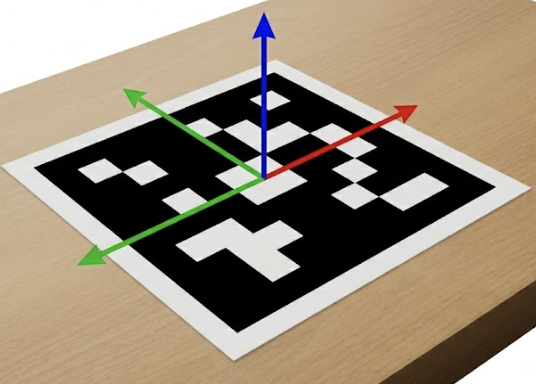
\includegraphics[width=0.6\textwidth]{Imagenes/Vectorial/codigoAruco.png}
    \caption{Ejemplo de marcador ArUco del diccionario 4$\times$4. El patrón binario interior codifica el identificador del marcador; el borde negro exterior facilita la detección del contorno.}
    \label{fig:codigoAruco}
\end{figure}

\subsection{Offsets de posición y rotación}

Incluso con una calibración precisa pueden existir pequeños desvíos visuales debidos a la tolerancia de impresión del marcador, imperfecciones en el plano donde está pegado o desajustes entre el centro geométrico del modelo 3D y el del patrón ArUco. Para solucionarlo, el plugin ofrece controles de \textit{offset} que el operador puede ajustar en directo:

\begin{itemize}
    \item \textbf{Posicionamiento manual (X, Y, Z):} Desplaza el modelo respecto al centro del marcador en las tres dimensiones. Permite centrar con precisión el objeto aunque su origen geométrico no coincida exactamente con el centro del ArUco.
    \item \textbf{Rotación manual (Pitch, Yaw, Roll):} Corrige la orientación del modelo. Es especialmente útil cuando el marcador está pegado sobre una superficie inclinada y el modelo aparece girado respecto a la vertical esperada.
    \item \textbf{Escala:} Factor de escala global del modelo, que el operador ajusta para que el tamaño del objeto virtual sea visualmente coherente con el tamaño físico del marcador y el entorno de la retransmisión.
\end{itemize}

Todos estos offsets se aplican sobre el stack de matrices del frame siguiente de forma inmediata, y se persisten automáticamente en el archivo de configuración de la escena de OBS al cerrar, de modo que la próxima vez que se cargue la escena el alineamiento sea idéntico.

\subsection{Modos de visualización}

El plugin ofrece cuatro modos de operación seleccionables desde el panel de propiedades, pensados para cubrir los distintos momentos de una retransmisión de concurso:

\begin{itemize}
    \item \textbf{Modelo 3D:} Modo estándar AR. Renderiza el modelo 3D cargado anclado al marcador configurado, con los offsets manuales aplicados.
    \item \textbf{Scoreboard:} Superpone sobre el marcador la tabla de clasificación general del concurso con los datos descargados de DOMjudge. No depende de ningún marcador específico; puede mostrarse en pantalla completa o anclado a un marcador de posición.
    \item \textbf{Team Info:} Muestra la información del equipo cuyo marcador la cámara está captando en ese instante. Cualquier marcador registrado en el fichero JSON de mapeo es válido.
    \item \textbf{Countdown (reloj):} Presenta el cronómetro 3D de cuenta atrás descrito en la sección anterior, con opción de anclarlo a un marcador ArUco o posicionarlo manualmente en pantalla.
\end{itemize}

Adicionalmente, el panel expone controles de visibilidad que permiten activar o desactivar capas de información (modelo 3D, overlays de texto, estado de conexión) de forma independiente sin interrumpir la emisión, lo que facilita la gestión en directo cuando la composición de la escena cambia durante el concurso.


\section{Conectividad y sincronización con DOMjudge}

Para que la realidad aumentada sea útil en un concurso de programación, el contenido virtual debe reflejar el estado real de la competición. El plugin integra un cliente especializado para comunicarse con \textbf{DOMjudge}, la plataforma líder en gestión de concursos de programación, y un sistema de sincronización asíncrona que mantiene los datos siempre actualizados sin interferir con el renderizado.

\begin{figure}[H]
    \centering
    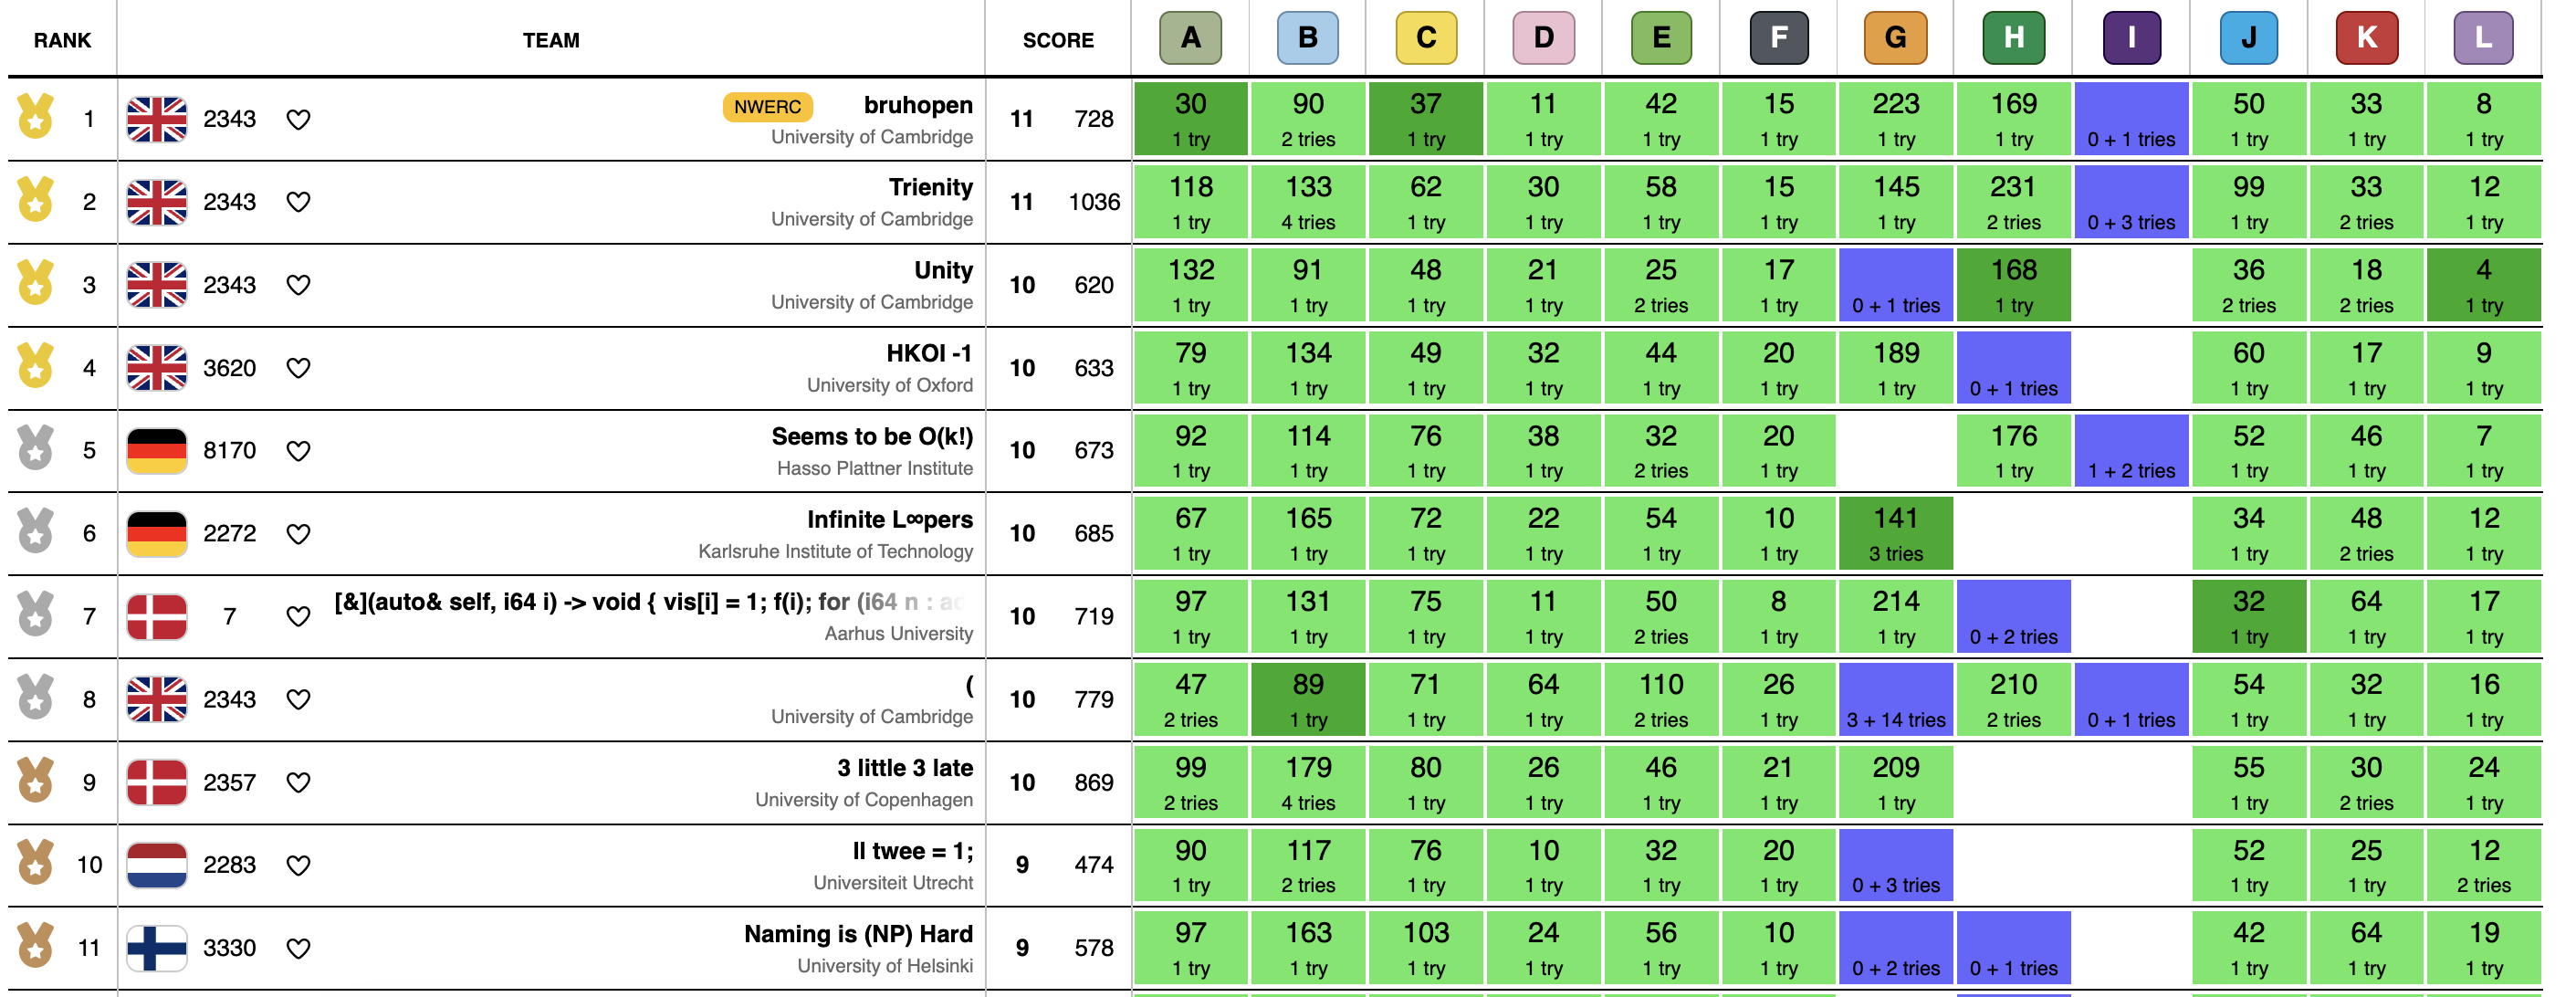
\includegraphics[width=0.6\textwidth]{Imagenes/Vectorial/juez2.png}
    \caption{Interfaz web de DOMjudge, cuya API REST es la fuente de datos del plugin.}
    \label{fig:domjudge_web}
\end{figure}

\subsection{Red asíncrona con libcurl}

Para evitar que la interfaz de OBS Studio se bloquee mientras se esperan datos del servidor, se ha implementado un módulo de red basado en la biblioteca \textbf{libcurl} que opera en el hilo secundario descrito en la sección~\ref{subsec:hilos}.

\begin{itemize}
    \item \textbf{Comunicación no bloqueante:} Las peticiones HTTP se realizan en el hilo secundario dedicado. El hilo principal de OBS nunca espera la respuesta del servidor; simplemente lee el último resultado disponible en la caché compartida cuando lo necesita.
    \item \textbf{Gestión de errores:} El sistema implementa políticas de \textit{timeout} y reintentos con espera exponencial. Si el servidor DOMjudge cae, el plugin sigue funcionando con los últimos datos guardados en caché, sin mostrar datos vacíos ni congelar la emisión.
\end{itemize}

\subsection{Máquina de estados de conexión}

La comunicación con el servidor se gestiona mediante una \textbf{máquina de estados} que garantiza la estabilidad del plugin incluso si la red falla:

\begin{itemize}
    \item \textbf{Activación binaria:} El operador puede desactivar la sincronización en cualquier momento para trabajar en modo local (\textit{offline}) con los datos en caché, por ejemplo durante una prueba de escenario sin conexión al servidor del concurso.
    \item \textbf{Estados de conexión:} El sistema transita entre \texttt{DISCONNECTED}, \texttt{CONNECTING}, \texttt{CONNECTED} y \texttt{FAILED}. El estado actual se muestra en el panel de OBS para que el operador sepa en todo momento si los datos son frescos o proceden de la caché.
    \item \textbf{Reintento automático (\textit{backoff}):} Si la conexión falla, el plugin no satura la red; espera intervalos crecientes antes de intentar reconectar, reduciendo la carga sobre el servidor en situaciones de sobrecarga.
\end{itemize}

\subsection{Configuración y seguridad}

El acceso a los datos de la competición requiere una configuración precisa del \textit{endpoint} remoto:

\begin{itemize}
    \item \textbf{Autenticación segura:} Se implementa soporte para \textit{HTTP Basic Auth}. Las credenciales se almacenan aprovechando la API de persistencia de OBS Studio, evitando que queden en texto plano en el archivo de configuración de la escena.
    \item \textbf{Identificación del torneo:} Parámetro que filtra los datos del servidor para obtener únicamente la información del evento actual mediante su ID de concurso en DOMjudge.
    \item \textbf{URL base:} Permite cambiar entre el servidor de producción del concurso y un entorno de prueba sin modificar el código fuente, simplemente actualizando el campo en el panel de propiedades.
\end{itemize}

\subsection{Endpoints y procesado JSON}

El plugin consulta periódicamente tres puntos clave de la API REST de DOMjudge para reconstruir el estado de la competición:

\begin{enumerate}
    \item \textbf{contests:} Obtiene metadatos como el nombre del torneo y el tiempo transcurrido y restante, vital para sincronizar el cronómetro 3D con la cuenta atrás oficial.
    \item \textbf{teams:} Descarga la lista de participantes, sus nombres reales y sus afiliaciones universitarias.
    \item \textbf{scoreboard:} Es el recurso más crítico. Proporciona el ranking actual, los problemas resueltos y el tiempo de penalización de cada equipo.
\end{enumerate}

El módulo \texttt{json\_utils} deserializa estas respuestas JSON y las convierte en estructuras de datos de lenguaje C, listas para ser consumidas por el motor de renderizado.

\subsection{Optimización de tráfico y latencia}

Dado que el plugin se ejecuta durante un \textit{streaming} que ya consume ancho de banda significativo, la eficiencia de red es un requisito de diseño:

\begin{itemize}
    \item \textbf{Intervalo de sincronización:} El operador configura cada cuántos segundos se consultan los datos. Un intervalo de 30 segundos es suficiente para mantener el scoreboard actualizado en la mayoría de concursos, equilibrando la frescura de la información con el consumo de datos.
    \item \textbf{Caché local:} Entre consultas, el plugin opera con los últimos datos recibidos. Esto garantiza que, aunque la red tenga picos de latencia, los overlays nunca muestran información vacía.
\end{itemize}

\subsection{Mapeo de marcadores a equipos}

La funcionalidad más innovadora del proyecto es el vínculo entre el mundo físico y los datos digitales. Esto se logra mediante una \textbf{tabla de mapeo} que el operador prepara en forma de fichero JSON antes de la retransmisión:

\begin{itemize}
    \item \textbf{Identificación unívoca:} Cada entrada del fichero asocia un ID de marcador ArUco con un ID de equipo en DOMjudge. Cuando la cámara detecta ese marcador, el plugin recupera automáticamente los datos del equipo correspondiente y los muestra como overlay.
    \item \textbf{Actualización en caliente:} El fichero JSON puede recargarse sin reiniciar la escena, lo que permite al operador corregir o ampliar el mapeo durante el propio concurso si fuera necesario.
\end{itemize}

\subsection{El \textit{scoreboard} visual}

Una vez obtenidos los datos de DOMjudge, el sistema los proyecta en el espacio virtual según el modo activo. El operador puede desplazar la tabla de puntuaciones en pantalla para evitar que tape elementos importantes del vídeo, y tiene la opción de anclarla a un marcador ArUco para que se posicione de forma automática en el espacio físico de la retransmisión. En el modo Scoreboard se presenta la clasificación general del concurso con posición, nombre del equipo, problemas resueltos y tiempo de penalización. En el modo Team Info el foco se centra en el equipo cuyo marcador la cámara está captando en ese instante, mostrando únicamente sus datos mientras el marcador sea visible.

%% ============================================================
%%  OVERLAY 2D SOBRE ARUCO: SCOREBOARD Y TEAM INFO
%% ============================================================


\section{Overlays 2D anclados al marcador}
\label{sec:overlays2d}

Los modos Scoreboard y Team Info comparten una misma arquitectura de renderizado cuyo propósito es diferente al del modelo 3D. En lugar de volumen y geometría, lo que se superpone al vídeo es un bloque de texto con información de la competición, diseñado para parecer físicamente anclado al marcador. El texto se mueve y rota con él cuando la cámara se desplaza, sin temblores perceptibles y sobre un fondo visualmente limpio. Lo que distingue a ambos modos entre sí es la fuente de datos y el criterio de detección del marcador, no el mecanismo de renderizado, que es común.

\subsection{El sistema de coordenadas}
\label{subsec:ydown}

Al combinar visión por computador con un motor gráfico surge casi inevitablemente un problema de convenios. OpenCV sitúa el origen de coordenadas en la esquina superior izquierda de la imagen con el eje $Y$ creciendo hacia abajo. La tradición de OpenGL, en cambio, coloca el origen abajo a la izquierda con el eje $Y$ hacia arriba. Si no se resuelve, cada posición que devuelve el detector aparece invertida verticalmente en pantalla.

\begin{figure}[h]
\centering
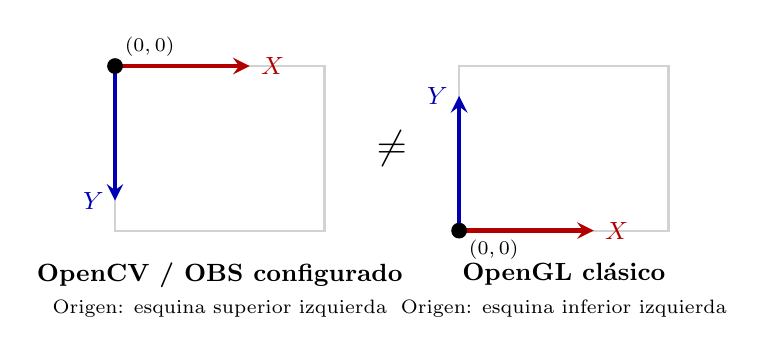
\begin{tikzpicture}[>=stealth, font=\small, scale=0.95]
  % OpenCV: origin top-left, Y down
  \draw[thick, gray!35] (0,0) rectangle (2.8,-2.2);
  \draw[->, ultra thick, red!70!black] (0,0) -- (1.8,0) node[right] {$X$};
  \draw[->, ultra thick, blue!70!black] (0,0) -- (0,-1.8) node[left] {$Y$};
  \fill (0,0) circle (3pt);
  \node[above right, font=\scriptsize] at (0,0) {$(0,0)$};
  \node[below, font=\small\bfseries] at (1.4,-2.5) {OpenCV / OBS configurado};
  \node[below, font=\scriptsize] at (1.4,-3.0) {Origen: esquina superior izquierda};
  % separator
  \node at (3.7,-1.1) {\Large$\neq$};
  % OpenGL: origin bottom-left, Y up
  \draw[thick, gray!35] (4.6,-2.2) rectangle (7.4,0);
  \draw[->, ultra thick, red!70!black] (4.6,-2.2) -- (6.4,-2.2) node[right] {$X$};
  \draw[->, ultra thick, blue!70!black] (4.6,-2.2) -- (4.6,-0.4) node[left] {$Y$};
  \fill (4.6,-2.2) circle (3pt);
  \node[below right, font=\scriptsize] at (4.6,-2.2) {$(0,0)$};
  \node[below, font=\small\bfseries] at (6.0,-2.5) {OpenGL clásico};
  \node[below, font=\scriptsize] at (6.0,-3.0) {Origen: esquina inferior izquierda};
\end{tikzpicture}
\caption{Convenios de coordenadas 2D. OBS se configura para usar el convenio de OpenCV, de forma que las coordenadas del detector se pueden usar sin transformación adicional.}
\label{fig:coordsystems}
\end{figure}

La solución adoptada fue configurar la proyección de OBS explícitamente con el convenio de OpenCV (origen en la esquina superior izquierda, eje $Y$ creciendo hacia abajo), de modo que las coordenadas del marcador se pueden usar directamente sin ninguna transformación adicional. Esto se traduce en que la llamada a la función de proyección ortográfica fija $y_{\min} = 0$ y $y_{\max} = H$ con el eje positivo apuntando hacia abajo, lo que garantiza:

\[
  x_{\text{render}} = x_{\text{detector}}, \qquad y_{\text{render}} = y_{\text{detector}}
\]

Esto elimina una fuente frecuente de errores y hace el código mucho más fácil de razonar.

Una consecuencia relevante de trabajar en proyección ortográfica es la gestión del rango de profundidad. El \textit{pipeline} de filtros de OBS opera exclusivamente en espacio 2D ortográfico: su API gráfica no expone un modo de proyección en perspectiva para filtros porque la salida de cada uno se composita como una textura plana. No existe un buffer de profundidad compartido entre fuentes, por lo que cualquier proyección en perspectiva quedaría aislada dentro del contexto del filtro sin integrarse con el resto de la composición. La rotación tridimensional del panel de texto se simula por tanto dentro de la proyección ortográfica mediante la cadena de matrices que se describe más adelante. El inconveniente es que, al aplicar rotaciones pronunciadas, los vértices del panel pueden alcanzar valores de profundidad fuera del rango por defecto, lo que hace que el plano de recorte (\textit{near/far clipping plane}) elimine parte de la geometría. Para evitarlo se configura la proyección con un rango deliberadamente amplio, de modo que ningún vértice del panel quede recortado aunque el marcador esté casi perpendicular a la cámara.

\subsection{El efecto visual buscado}
\label{subsec:objetivo_overlay}

El efecto buscado es que el bloque de texto parezca estar encima del marcador como una pantalla flotante sobre la mesa. Si el marcador está inclinado hacia la cámara, el texto se inclina con él. Si el marcador gira en el plano de la mesa, el texto gira también. Y si el operador mueve la cámara, el texto permanece centrado sobre el marcador en todo momento.

Para lograr esto, el sistema calcula en cada frame el centro geométrico del marcador en coordenadas de pantalla, promediando las posiciones de sus cuatro esquinas detectadas. Ese punto se convierte en el origen de toda la cadena de transformaciones que posicionará el texto. A partir de ahí se aplica la orientación real del marcador en el espacio, extraída por el algoritmo de estimación de pose, y un ajuste final que centra el bloque de texto sobre ese punto de anclaje. El usuario puede afinar el resultado con controles de offset de posición y rotación que actúan siempre sobre los ejes de la pantalla, independientemente de cómo esté orientado el marcador físico, lo que hace que su comportamiento sea intuitivo incluso para alguien que no conozca los detalles de la implementación.

\subsection{Detección en los modos de texto}
\label{subsec:deteccion_overlay}

La detección se ejecuta en el hilo de vídeo de OBS, separado del hilo de renderizado, de modo que el análisis de imagen no bloquea en ningún momento la salida visual. Cada frame que llega de la fuente de vídeo se convierte primero al espacio de color que OpenCV requiere y, una vez en escala de grises, se pasa al detector ArUco.

El detector localiza los marcadores presentes en la imagen y, para el elegido, calcula su posición y orientación tridimensional respecto a la cámara mediante el problema de Perspectiva-$n$-Puntos. La idea es:  si se sabe que el marcador es un cuadrado de tamaño conocido y se ven sus cuatro esquinas en la imagen, existe una única posición y orientación en el espacio que explicaría exactamente esa proyección. El resultado es un vector de traslación (a qué distancia y en qué dirección está el marcador) y un vector de rotación (cómo está orientado en el espacio).

Las coordenadas en píxeles de las esquinas se escalan a la resolución de salida de OBS de forma proporcional:

\[
  s_x = \frac{W_{\text{base}}}{W_{\text{frame}}}, \qquad s_y = \frac{H_{\text{base}}}{H_{\text{frame}}}
\]

donde $W_{\text{base}} \times H_{\text{base}}$ es la resolución base de la escena OBS y $W_{\text{frame}} \times H_{\text{frame}}$ la del frame capturado. Este escalado garantiza que las posiciones del marcador sean siempre coherentes con el espacio en que se dibuja el overlay, independientemente de la resolución real de la cámara.

\subsubsection{Conversión de formatos de vídeo de entrada}
\label{subsubsec:formatos}

OBS puede entregar frames en múltiples formatos de píxel según la fuente de vídeo conectada. Antes de cualquier análisis, el módulo de detección convierte el frame al espacio de color BGR que OpenCV requiere. La Tabla~\ref{tab:formatos_video} resume los formatos soportados y la estrategia de conversión aplicada en cada caso.

\begin{table}[H]
\centering
\renewcommand{\arraystretch}{1.2}
\begin{tabular}{|l|l|p{5.5cm}|}
\hline
\textbf{Formato OBS} & \textbf{Tipo} & \textbf{Conversión a BGR} \\
\hline
\texttt{I420}            & YUV 4:2:0 planar      & Planos Y, U, V separados. \texttt{cvtColor(YUV2BGR\_I420)}. \\
\texttt{NV12}            & YUV 4:2:0 semi-planar & Plano Y + UV entrelazado. \texttt{cvtColor(YUV2BGR\_NV12)}. \\
\texttt{YUY2/YUYV}       & YUV 4:2:2 empaquetado & Patrón Y0 U0 Y1 V0. \texttt{cvtColor(YUV2BGR\_YUY2)}. \\
\texttt{UYVY}            & YUV 4:2:2 empaquetado & Variante con crominancia adelantada. \texttt{cvtColor(YUV2BGR\_UYVY)}. \\
\texttt{BGRA}            & RGB directo 32 bits   & Descarte del canal alfa. Copia directa del buffer. \\
\texttt{RGBA}            & RGB directo 32 bits   & Reordenación de canales $R \leftrightarrow B$. \\
\texttt{Y800 / Y8}       & Escala de grises      & Ya en el formato final. Se usa directamente. \\
\hline
\end{tabular}
\caption{Formatos de vídeo soportados por el módulo de detección y su conversión a BGR para OpenCV.}
\label{tab:formatos_video}
\end{table}

Las conversiones YUV utilizan la fórmula estándar BT.601, donde cada componente de color se obtiene a partir de la luminancia $Y$ y las crominancias $U$ (diferencia de azul) y $V$ (diferencia de rojo):

\[
  R = Y + 1.403\,V', \quad G = Y - 0.344\,U' - 0.714\,V', \quad B = Y + 1.770\,U'
\]

con $U' = U - 128$ y $V' = V - 128$ como valores de crominancia centrados en cero. Una vez obtenida la imagen BGR, se convierte a escala de grises con una ponderación perceptual estándar antes de pasarla al detector.

\subsubsection{De la rotación detectada a la orientación del overlay}
\label{subsubsec:rodrigues}

La orientación que devuelve el algoritmo viene en un formato llamado representación de Rodrigues: un único vector donde la dirección indica el eje alrededor del que gira el marcador y la longitud indica cuánto gira. Es una forma compacta y sin ambigüedades de codificar cualquier rotación en el espacio, pero para orientar el overlay se necesita traducirla a algo que OBS pueda aplicar directamente. El proceso sigue el siguiente pipeline:

\vspace{0.6cm}
\begin{figure}[h]
\centering
\begin{tikzpicture}[
    node distance=0.6cm and 1.1cm,
    box/.style={rectangle, rounded corners=4pt, draw=black!60, fill=gray!10,
                minimum width=2.6cm, minimum height=0.9cm, align=center, font=\small},
    arr/.style={->, thick, >=stealth}
  ]
  \node[box] (rvec)  {\textbf{rvec}\\\scriptsize vector Rodrigues\\$(r_x, r_y, r_z)$};
  \node[box, right=of rvec] (R)    {\textbf{Matriz R}\\\scriptsize rotación $3\times3$};
  \node[box, right=of R]    (euler){\textbf{Euler}\\\scriptsize pitch, yaw, roll};
  \node[box, right=of euler] (pose) {\textbf{Pose}\\\scriptsize orientación\\del overlay};
  \draw[arr] (rvec)  -- node[above, font=\scriptsize] {Rodrigues} (R);
  \draw[arr] (R)     -- node[above, font=\scriptsize] {extracción} (euler);
  \draw[arr] (euler) -- node[above, font=\scriptsize] {aplicación} (pose);
\end{tikzpicture}
\caption{Pipeline de conversión de la representación de Rodrigues a la orientación del overlay.}
\label{fig:rodrigues_pipeline}
\end{figure}

El módulo de detección convierte esa representación a una matriz de rotación $3\times3$ que describe cómo están orientados los tres ejes del marcador respecto a la cámara. De esa matriz se extraen los ángulos de inclinación hacia delante y hacia los lados (pitch y yaw) y el giro sobre el propio eje (roll), que son los que finalmente guían cómo se orienta el panel de texto en el espacio 3D de OBS. Cuando el marcador se inclina extremadamente existe un caso matemático conocido como \textit{gimbal lock} donde dos de los tres ángulos se vuelven dependientes y no se pueden distinguir por separado. El sistema detecta esta situación y aplica un cálculo alternativo para evitar comportamientos extraños en el overlay.

Adicionalmente, el módulo calcula en qué dirección apunta la cara del marcador proyectada sobre la imagen de la cámara. Esto sirve para que el texto siempre resulte legible: aunque el marcador esté ligeramente girado en el plano de la mesa, el sistema ajusta la orientación del overlay para que el texto no quede volcado o boca abajo.

\subsection{Selección y mapeo de marcadores en Team Info}
\label{subsec:seleccion_marcador}

El modo Team Info requiere saber qué equipo corresponde a cada marcador físico impreso en las mesas del concurso. Esta asociación se define en un fichero JSON que el operador prepara antes de la retransmisión:

\begin{verbatim}
[
  { "marker_id": 1, "team_id": "42" },
  { "marker_id": 2, "team_id": "12" },
  { "marker_id": 5, "team_id": "7"  }
]
\end{verbatim}

Al cargar el fichero, el módulo de sincronización construye en memoria la tabla de mapeos y extrae la lista compacta de todos los IDs de marcador válidos. Esa lista es la que recibe el módulo de detección para que, en cada frame, filtre los marcadores detectados y descarte los que no corresponden a ningún equipo registrado.

En cuanto a la selección cuando hay varios marcadores simultáneos en pantalla: en el modo Scoreboard el sistema busca un único marcador con el ID configurado. En el modo Team Info cualquier marcador del fichero JSON es válido, y si aparecen varios a la vez el sistema elige el primero en el orden en que el detector los devuelve, que corresponde al orden natural de aparición en la imagen. Este comportamiento es simple y predecible: en una retransmisión habitual la cámara apunta a un equipo concreto, por lo que la ambigüedad rara vez se presenta. Si en algún momento se necesitara mostrar varios equipos simultáneamente, basta con añadir una instancia del filtro por equipo, cada una configurada para su marcador correspondiente, trabajando en paralelo sin interferencias.

Una vez identificado el marcador, el sistema cruza su ID con la tabla de mapeo para obtener el identificador del equipo y recupera sus datos de la caché local, actualizada periódicamente desde DOMjudge. Si el equipo está en caché, su información (nombre, posición en el ranking, problemas resueltos y tiempo de penalización) se vuelca en el bloque de texto del overlay y se renderiza con el mecanismo de posicionamiento descrito en las secciones anteriores.

\subsection{Composición del scoreboard}
\label{subsec:multicolumna}

El modo Scoreboard organiza la información en cuatro columnas: posición, nombre del equipo, problemas resueltos y tiempo de penalización. Cada columna es una fuente de texto de OBS independiente, lo que permite controlar el estilo visual de cada una por separado (tamaño de fuente, color, negrita) y que sus anchos se adapten automáticamente al contenido real en cada momento, sin riesgo de que un nombre largo desborde o quede truncado artificialmente.

El ancho total del bloque se calcula sumando los anchos reales de las cuatro columnas más tres separadores fijos:

\[
  T_w = W_{\text{pos}} + W_{\text{nombre}} + W_{\text{res}} + W_{\text{tiempo}} + 3\,\delta, \qquad \delta = 18\;\text{px}
\]

Las cuatro columnas se dibujan en secuencia de izquierda a derecha, avanzando un cursor horizontal $x_c$ que se actualiza tras cada columna renderizada:

\[
  x_c^{(k+1)} = x_c^{(k)} + W_k + \delta, \quad k = 0, 1, 2, 3
\]

El resultado visual es una tabla compacta que, al estar todas sus columnas bajo la misma transformación AR, se mueve y rota como un bloque único cuando está anclada al marcador.

\subsection{Cadena de transformaciones}
\label{subsec:pipeline_matrices}

Anclar el bloque de texto al marcador con la orientación correcta requiere encadenar varias transformaciones en un orden muy preciso. La API gráfica de OBS gestiona estas transformaciones mediante un stack acumulativo: cada nueva operación se combina con todas las anteriores y el vértice final recibe el resultado completo.

La transformación total que recibe cada vértice del overlay es:

\[
  M = T_{\text{pos}} \cdot R_{\text{offsets}} \cdot R_{\text{flip}} \cdot R_{\text{ArUco}} \cdot R_{\text{elev}} \cdot T_{\text{centrado}}
\]

Cada factor tiene un papel concreto. $T_{\text{pos}}$ traslada el origen de dibujo al centro del marcador en pantalla, incorporando el offset de posición configurado por el usuario. $R_{\text{offsets}}$ aplica los offsets de rotación manuales sobre los ejes de pantalla (inclinación, giro lateral, giro en profundidad) de forma predecible e independiente de la orientación del marcador. $R_{\text{flip}}$ corrige la diferencia de convenios entre OpenCV y OBS mediante una rotación de $180°$ sobre el eje horizontal:

\[
  R_{\text{flip}} = R_x(180°) =
  \begin{pmatrix} 1 & 0 & 0 \\ 0 & -1 & 0 \\ 0 & 0 & -1 \end{pmatrix}
\]

Esta matriz invierte los ejes $Y$ y $Z$, lo que implica que el vector de rotación ArUco $\vec{r} = (r_x,\, r_y,\, r_z)$ debe expresarse con sus componentes $Y$ y $Z$ negadas al aplicarlo en espacio OBS:

\[
  \vec{r}_{\,\text{OBS}} = \bigl(r_x,\; -r_y,\; -r_z\bigr)
\]

$R_{\text{ArUco}}$ aplica la rotación real del marcador detectada por el algoritmo PnP: es la que hace que el texto se incline y gire cuando lo hace el marcador físico. $R_{\text{elev}}$ añade una rotación de $90°$ sobre el eje horizontal para que el panel quede erguido sobre el marcador en lugar de tumbado sobre él:

\[
  R_{\text{elev}} = R_x(90°) =
  \begin{pmatrix} 1 & 0 & 0 \\ 0 & 0 & -1 \\ 0 & 1 & 0 \end{pmatrix}
\]

Por último, $T_{\text{centrado}}$ desplaza el bloque la mitad de su ancho hacia la izquierda y su altura completa hacia arriba, de modo que quede centrado horizontalmente sobre el marcador y crezca hacia arriba desde el punto de anclaje.

\subsection{Suavizado del overlay}
\label{subsec:suavizado}

Aunque la detección ArUco es robusta, el ruido de la imagen de cámara, como el granulado del sensor, la compresión de vídeo o las microvibraciones, provoca que la posición y el ángulo calculados del marcador oscilen ligeramente de frame a frame. Sin ninguna corrección, el texto parece temblar sobre el vídeo, lo que resulta poco profesional en una retransmisión.

Para mitigarlo, el sistema aplica un filtro de suavizado exponencial sobre la posición y el ángulo del overlay. En lugar de saltar directamente al valor nuevo detectado en cada frame, se mezcla ese valor nuevo con el del frame anterior según un factor configurable $\alpha \in (0,\,1]$:

\[
  P_t = (1 - \alpha)\,P_{t-1} + \alpha\,P_{\text{detectado}}
\]

Con $\alpha$ cercano a $1$ el overlay sigue el marcador con mucha fidelidad pero puede mostrar algo de temblor residual. Con $\alpha$ más pequeño el movimiento es más suave pero tiene algo más de inercia, por lo que en cámara rápida puede quedarse ligeramente retrasado. El operador ajusta este parámetro según las condiciones de grabación.

El ángulo requiere un tratamiento especial. Si el marcador pasa de estar a $179°$ a $-179°$, una interpolación directa haría girar el overlay $358°$ en sentido contrario en lugar de $2°$. El sistema detecta este caso y siempre interpola por el camino angular más corto entre los dos valores. El suavizado se reinicia automáticamente cuando el marcador detectado cambia de ID, para no arrastrar la posición del marcador anterior a la animación del nuevo.

\subsection{Fondo del overlay}
\label{subsec:rounded}

Para mejorar la legibilidad del texto sobre vídeo en movimiento, el sistema puede dibujar un fondo semitransparente detrás del bloque de texto, con esquinas redondeadas y una sombra opcional.

El fondo es un rectángulo con las esquinas suavizadas en arco. En lugar de ángulos rectos, cada esquina se redondea con un radio configurable, lo que da al panel un aspecto más limpio y lo hace visualmente más agradable sobre el vídeo, especialmente cuando el fondo de imagen cambia entre frames. Esta forma se calcula una sola vez cuando el bloque de texto cambia de tamaño y se almacena directamente en la memoria de la tarjeta gráfica, de modo que en cada frame no hay que recalcular nada: la geometría ya está lista para dibujar.

La sombra se consigue dibujando ese mismo fondo varias veces, cada vez ligeramente desplazado respecto al anterior y con un poco menos de opacidad. El resultado es que el panel parece flotar sobre el vídeo con un halo difuso debajo, dando sensación de profundidad sin necesidad de ningún procesado especial de imagen ni de shaders adicionales. Es una técnica deliberadamente sencilla: varias pasadas del mismo dibujo con parámetros de color y posición distintos, lo que la hace eficiente y fácil de ajustar cambiando únicamente el número de pasadas y la intensidad de cada una.


\section{Liberación de recursos}

Un aspecto crítico en el desarrollo de plugins para OBS Studio es la gestión del ciclo de vida de los recursos. Debido a que el plugin puede activarse y desactivarse dinámicamente, es imperativo garantizar una limpieza absoluta para evitar fugas de memoria (\textit{memory leaks}) que degraden el rendimiento del sistema anfitrión.

\subsection{Persistencia de estado}

Antes del cierre definitivo, el plugin realiza dos tareas finales de integridad:
\begin{enumerate}
    \item \textbf{Limpieza de Credenciales:} Por seguridad, las contraseñas de la API se sobrescriben en memoria antes de ser liberadas, evitando que queden trazas en el \textit{heap} del proceso.
    \item \textbf{Guardado de Configuración:} Los \textit{offsets} y ajustes realizados por el usuario durante la sesión se persisten en el archivo de configuración de la escena de OBS, permitiendo que la próxima vez que se cargue el plugin, el alineamiento sea idéntico.
\end{enumerate}

\subsection{Memoria GPU}

Los recursos gráficos residen en la memoria de la tarjeta de vídeo y su liberación debe estar sincronizada con el hilo de renderizado de OBS:

\begin{itemize}
    \item \textbf{Destrucción de Buffers:} Al desactivar el plugin, se invocan de forma recursiva las funciones de destrucción de los \textit{Vertex Buffer Objects} (VBO) y los \textit{Index Buffers}. Se sigue un orden estricto para evitar accesos a memoria inválida.
    \item \textbf{Limpieza de Texturas:} Las imágenes cargadas para los modelos 3D y el reloj se eliminan de la VRAM. Se utiliza un sistema de conteo de referencias para asegurar que una textura compartida solo se borre cuando ningún objeto la necesite.
\end{itemize}

\subsection{Limpieza del detector}

El detector ArUco mantiene estructuras pesadas que deben cerrarse ordenadamente:
\begin{itemize}
    \item \textbf{Estructuras de OpenCV:} Se liberan los diccionarios de marcadores y las matrices de calibración de cámara para devolver la memoria al sistema.
    \item \textbf{Seguimiento Temporal:} Se reinicializan los filtros de suavizado y las últimas poses conocidas, garantizando que si el plugin se vuelve a activar, comience desde un estado limpio sin heredar posiciones antiguas.
\end{itemize}

\subsection{Cierre de conexiones}

El módulo de sincronización web gestiona recursos externos que requieren una finalización controlada. Si hay una petición a DOMjudge en curso al cerrar el plugin, el sistema señaliza al hilo secundario que debe detenerse, espera a que termine limpiamente y cierra los sockets TCP abiertos. A continuación se liberan todas las estructuras de datos que contienen el scoreboard, la lista de equipos, los resultados de los problemas y la tabla de mapeo de marcadores, recorriendo los arrays dinámicos de forma recursiva hasta dejar la memoria completamente limpia.

